\documentclass[letterpaper]{article}
\usepackage{aaai25}
\usepackage{times}
\usepackage{helvet}
\usepackage{courier}
\usepackage[hyphens]{url}
\usepackage{graphicx}
\urlstyle{rm}
\def\UrlFont{\rm}
\usepackage{natbib}
\usepackage{caption}
\frenchspacing
\setlength{\pdfpagewidth}{8.5in}
\setlength{\pdfpageheight}{11in}

\usepackage{amsmath,amssymb}
\usepackage{algorithm}
\usepackage{algorithmic}
\usepackage{booktabs}
\usepackage{multirow}
\usepackage{pifont}
\usepackage{tikz}
\usetikzlibrary{shapes,arrows,positioning,fit,backgrounds}

\pdfinfo{
/TemplateVersion (2025.1)
}

\setcounter{secnumdepth}{0}

\title{Trust Before Reuse: Contracted Counterfactual Certification of \\ Self-Evolved Knowledge in Minecraft Agents}

\author{
    Anonymous Author(s)\\
    Anonymous Affiliation\\
    Anonymous Email
}

\begin{document}

\maketitle

\begin{abstract}
Self-evolving agents in open-world environments continuously accumulate experience-derived knowledge. Yet the decision of \emph{whether to reuse} this knowledge at decision time has received almost no direct study: existing consolidation gates evaluate surface features---success counts, format validity, semantic similarity---without measuring whether the knowledge \emph{causes} improved outcomes when actually deployed. We argue that knowledge reuse permission is fundamentally a counterfactual question---what would have happened had we used the base policy instead?---and that answering it requires a structured framework combining causal measurement, statistical calibration, and verifiable behavioral claims. We propose \textsc{C-ACT} (Contracted Adaptive Counterfactual Trust), a lightweight decision-time admission layer that introduces three innovations: (1)~a \emph{Knowledge Contract} schema that transforms unstructured self-evolved knowledge into falsifiable behavioral claims with explicit preconditions, postconditions, expected uplift, and hard safety boundaries; (2)~a \emph{Bayesian counterfactual gate} that maintains three Beta posteriors per knowledge item (success-when-used, success-when-skipped, harmful-reuse-rate) and computes the exact posterior probability that reuse improves outcomes beyond an adaptively calibrated threshold; and (3)~an \emph{adaptive lifecycle governance} system with a six-state state machine and a novel supervised-reuse regime for probation-phase knowledge. \textsc{C-ACT} is not a skill generator nor a knowledge-bank curator---it is a decision-time admission layer compatible with any knowledge generation and retrieval pipeline. We instantiate \textsc{C-ACT} on \textsc{XENON}'s experience-corrected dependency and action knowledge in Minecraft, comparing seven gate designs across 36 tasks under strict frozen evaluation with eight seeds. \textsc{C-ACT} reduces harmful reuse rate by 62\% over retrieve-and-reuse baselines, improves hard-task success rate by 18pp, and achieves 14--20pp higher coverage at equivalent risk budgets compared to fixed-threshold Bayesian gates. Online evolution experiments over five accumulation rounds demonstrate that \textsc{C-ACT}'s lifecycle governance prevents knowledge pollution, maintaining a stable certified knowledge ratio while no-gate baselines degrade after Round~3. Ablation confirms that the Knowledge Contract and adaptive calibration are the two largest contributors, jointly accounting for over 70\% of the performance gain.
\end{abstract}

\section{Introduction}

An autonomous agent operating in an open-world environment like Minecraft faces a fundamental knowledge management problem. After successfully completing a task---or failing and recovering---the agent can extract structured knowledge from the experience: a dependency correction (``furnace crafting requires cobblestone, not stone''), an action correction (``mine diamond with iron pickaxe, never stone''), or a failure remedy (``if smelting fails, check that fuel is present''). This knowledge is intended to improve future performance in similar situations.

The dominant paradigm in self-evolving agents is to apply a \emph{heuristic gate} that decides whether this knowledge is worth keeping or reusing~\cite{voyager2023,mineevolve2026,peam2026}. PEAM~\cite{peam2026}, the state-of-the-art in parametric experience consolidation for Minecraft, uses a four-dimensional weighted sum (PV score) combining estimated cost savings, stability, redundancy avoidance, and forgetting risk. MineEvolve~\cite{mineevolve2026} employs a five-rule Curator checking schema validity, execution consistency, and conflict patterns. These heuristics ask variants of the question ``does this knowledge look good?''---evaluating surface features of the knowledge itself or its source episode.

We argue that this question is fundamentally misaligned with the actual decision problem. The correct question is: \textbf{``does reusing this knowledge \emph{cause} better outcomes than not reusing it, in this specific context?''} This is a counterfactual question---it requires comparing what happens \emph{with} the knowledge to what would have happened \emph{without} it. A knowledge item may exhibit high success rates in its source episodes due to initial inventory advantages, planner capability, or environmental shortcuts, none of which generalize to new contexts~\cite{mineexplorer2025}. Conversely, statistically successful knowledge may interfere with previously mastered same-category skills when reused---a phenomenon we term \emph{passive interference}. No prior work has directly measured the causal effect of reusing a specific piece of self-evolved knowledge on downstream task outcomes.

This gap is structural, not incremental. It stems from conflating two distinct problems: (1)~knowledge \emph{generation}---what knowledge exists? (2)~knowledge \emph{retrieval}---what knowledge is relevant? (3)~knowledge \emph{admission}---should this knowledge affect behavior now? Existing work has thoroughly studied (1) and (2); (3) has been treated as an afterthought, collapsed into the same heuristic that governs generation or retrieval. We argue that admission is a first-class problem requiring its own dedicated mechanism.

We propose \textbf{\textsc{C-ACT}} (Contracted Adaptive Counterfactual Trust), a decision-time admission layer for self-evolved knowledge. \textsc{C-ACT} is \emph{not} a skill generator, \emph{not} a knowledge-bank curator, and \emph{not} an alternative to retrieval. It is a thin governance layer that sits between retrieval and execution, answering one question: ``Is this already-retrieved knowledge permitted to affect the next action?''

\textsc{C-ACT} makes three contributions:

\begin{enumerate}
    \item \textbf{Knowledge Contract}: Self-evolved knowledge is transformed from unstructured text into falsifiable behavioral claims. Each contract specifies preconditions that must hold before reuse, postconditions that must hold after, expected uplift, a declared risk bound, and---critically---hard safety boundaries (non-applicable contexts such as lava, combat, or low health) where reuse is unconditionally forbidden regardless of statistical evidence. Contracts make knowledge \emph{auditable}: every reuse decision can be traced to specific precondition checks, and every violation is logged.

    \item \textbf{Bayesian Counterfactual Gate with Adaptive Calibration}: For each knowledge item $u$ in context $c$, \textsc{C-ACT} maintains three Beta posteriors---$p_{\text{use}}$ (success when knowledge is used), $p_{\text{base}}$ (success when the base/fallback policy is used instead), and $p_{\text{harm}}$ (harmful reuse probability). The core decision statistic is the \emph{Bayesian counterfactual uplift probability}: $\pi_u(c) = P(p_{\text{use}} > p_{\text{base}} + \delta \mid \mathcal{D})$. Reuse is permitted only when all four conditions hold: (i)~$\pi_u(c) \ge \tau^\star_{g,l}$, (ii)~$h_u^+(c) \le h^\star_{g,l}$, (iii)~contract preconditions are satisfied, and (iv)~no pairwise interaction conflict is detected. The thresholds $(\tau^\star, \delta^\star, h^\star)$ are \emph{not} hand-tuned---they are learned per task group and knowledge level via constrained optimization on a held-out calibration set, maximizing coverage subject to a pre-specified risk budget $\epsilon_{\text{harm}} = 0.10$.

    \item \textbf{Adaptive Lifecycle Governance with Supervised Reuse}: Knowledge transitions through a six-state lifecycle (Candidate $\rightarrow$ Quarantined $\rightarrow$ Probation $\rightarrow$ Certified $\rightarrow$ Deprecated $\rightarrow$ Disabled) based on accumulating evidence, contract compliance, and drift detection. A key innovation is the \textbf{supervised reuse} regime for Probation-phase knowledge: it has sufficient evidence to suggest benefit (3--5 observations, $\pi_u > 0.3$) but the posterior is still wide. Rather than blocking all Probation knowledge (which would increase false negatives and harm success rate) or granting unrestricted reuse (which would risk harmful reuse), \textsc{C-ACT} permits supervised reuse with mandatory reflection verification after each execution step. This design reduces the false-negative rate while maintaining safety.
\end{enumerate}

We evaluate \textsc{C-ACT} on \textsc{XENON}'s~\cite{xenon2024} experience-corrected dependency and action knowledge in Minecraft, comparing seven gate designs across 36 tasks from MCU-turbo~\cite{mcu2024} and MineDojo~\cite{minedojo2022} under strict frozen evaluation with eight seeds. Empirical results demonstrate: (1)~a 62\% reduction in harmful reuse rate (HRR) over retrieve-and-reuse baselines; (2)~14--20pp higher coverage at equivalent risk budgets compared to fixed-threshold Bayesian gates; (3)~a monotonic success rate increase across five online evolution rounds, while no-gate baselines degrade after Round~3 due to knowledge pollution. Ablation confirms that the Knowledge Contract and adaptive calibration jointly account for over 70\% of \textsc{C-ACT}'s performance gain, and that exploration tasks show no significant difference across methods---a positive control confirming that \textsc{C-ACT}'s benefit is specific to its claimed mechanism.

\section{Related Work}

\subsection{Self-Evolving Agents and Experience Consolidation}

The progression from LLM-based planning to experience-driven self-evolution in Minecraft agents has been rapid. Voyager~\cite{voyager2023} introduced the paradigm of an executable code skill library with automatic curriculum, demonstrating that LLM-generated programs could accumulate into reusable assets. DEPS~\cite{deps2023} and MP5~\cite{mp52024} refined the planning-execution-reflection loop with hierarchical task decomposition and multimodal feedback. These systems generate knowledge (skills, plans) but apply no admission control---all generated skills are stored and retrieved without gating.

Subsequent work introduced explicit consolidation decisions. MineEvolve~\cite{mineevolve2026} converts typed execution feedback into skill/remedy pairs, with a five-rule Curator checking format validity, execution repeatability, conflict patterns, and schema consistency. PEAM~\cite{peam2026} takes the most aggressive approach: it trains micro-LoRA adapters from successful and failure-correction trajectories and uses a four-dimensional PV score (cost saving, stability, redundancy, forgetting) to select which adapters to consolidate into parametric memory. EvolvingAgent~\cite{evolvingagent2025} uses curriculum learning to select experiences for world-model updates. Echo~\cite{echo2026} decomposes transfer similarity across five axes (structural, attributive, procedural, functional, interactional) to decide when knowledge from one task applies to another.

Table~\ref{tab:gates} characterizes the gate problem across these systems. Every existing gate evaluates \emph{intrinsic properties} of the knowledge or its source episode---none measures the causal effect of reusing the knowledge in a new context. This is the gap \textsc{C-ACT} addresses.

\begin{table}[t]
\centering
\caption{Comparison of consolidation/reuse gates in self-evolving agents. All existing gates are heuristic; none measures counterfactual effect.}
\label{tab:gates}
\small
\begin{tabular}{lccccc}
\toprule
\textbf{System} & \textbf{Gate Type} & \textbf{Features} & \textbf{Counts} & \textbf{Measures} & \textbf{Counter-} \\
& & \textbf{Used} & \textbf{Success?} & \textbf{Interference?} & \textbf{factual?} \\
\midrule
Voyager~\cite{voyager2023} & None (all stored) & --- & --- & --- & --- \\
MineEvolve~\cite{mineevolve2026} & 5-rule static & Schema, conflict & \ding{51} & \ding{51} & \ding{55} \\
PEAM~\cite{peam2026} & 4-dim weighted sum & Heuristic PV & \ding{51} & Partial & \ding{55} \\
Echo~\cite{echo2026} & 5-axis similarity & Transfer axes & \ding{51} & \ding{55} & \ding{55} \\
\textbf{C-ACT} (ours) & Adaptive Bayesian & $\pi_u, h^+$, contract & \textbf{\ding{51}} & \textbf{\ding{51}} & \textbf{\ding{51}} \\
\bottomrule
\end{tabular}
\end{table}

\subsection{Causal Methods for Agent Memory}

Recent work has begun applying causal reasoning to agent memory, primarily at inference time. CMI~\cite{cmi2026} estimates the causal effect of individual dialogue turns in long-context LLM interactions to select which memories to include in prompts. CausalFlow~\cite{causalflow2026} performs step-level failure attribution in tool-use and reasoning chains. WISE~\cite{wise2026} constructs causal event graphs over spatial and temporal knowledge for retrieval scheduling. These methods intervene on \emph{prompt composition}---deciding which text to include in the LLM context. \textsc{C-ACT} intervenes one level earlier: on \emph{policy behavior}---deciding whether retrieved knowledge should be allowed to shape the agent's next action. The intervention target differs (prompt vs.~policy), the outcome metric differs (answer quality vs.~task success and harm), and \textsc{C-ACT} additionally enforces safety constraints that are absent from prompt-level selection methods.

\subsection{Bayesian Decision-Making and Conformal Methods}

Bayesian methods have been applied to agent decision problems including bandit-based tool selection~\cite{ael2026} and confidence-calibrated planning~\cite{ccp2026}. \textsc{C-ACT}'s TrustStore uses Beta-Bernoulli conjugate updates for computational efficiency---each observation requires only two floating-point additions. The TrustGate's calibration procedure connects to conformal prediction~\cite{conformal}: given a held-out calibration set, we search for threshold configurations that maximize coverage subject to a finite-sample risk bound. However, \textsc{C-ACT}'s gate is a batch calibration procedure rather than online conformal prediction; the thresholds are fixed after E2 calibration and applied without further update during E3 evaluation. We use empirical Bernstein bounds~\cite{anytime} for the finite-sample risk upper bound during calibration.

\section{Problem Formulation}

\subsection{Decision-Time Knowledge Admission}

Let $\mathcal{K} = \{u_1, \ldots, u_K\}$ be a knowledge store generated by an upstream pipeline (e.g., \textsc{XENON}'s Adaptive Dependency Graph or Failure-aware Action Memory). At decision time $t$, given current state $s_t$ and context $c_t$, a subset $\mathcal{R}_t \subseteq \mathcal{K}$ is retrieved as candidate knowledge. The admission problem is to assign a binary decision to each candidate:

\begin{equation}
\label{eq:admission}
\text{admit}: \mathcal{K} \times \mathcal{C} \rightarrow \{0, 1\}
\end{equation}

where $\text{admit}(u, c_t) = 1$ means knowledge $u$ is permitted to influence the agent's behavior in context $c_t$, and $\text{admit}(u, c_t) = 0$ means the agent falls back to its base policy $\pi_{\text{base}}$ for decisions involving $u$.

This is neither the generation problem (which knowledge items exist) nor the retrieval problem (which items are relevant). It is a distinct governance decision: relevance and prior success are necessary but insufficient conditions for admission.

\subsection{Constrained Optimization Objective}

The admission policy $\pi$ must optimize a dual objective:

\begin{equation}
\label{eq:objective}
\max_{\pi} \; \mathbb{E}_{u,c}\left[\text{Success} \mid \text{admit}_\pi(u,c) = 1\right] \quad \text{s.t.} \quad P(\text{harmful} \mid \text{admit}_\pi(u,c) = 1) \leq \epsilon_{\text{harm}}
\end{equation}

where $\epsilon_{\text{harm}} = 0.10$ is the pre-declared safety budget. Harmful reuse is defined strictly as either (i)~progress regression with cost exceeding budget: $\Delta\text{progress} \leq 0 \land \text{Cost} > B$, or (ii)~an unrecoverable failure event that terminates the episode.

The optimization in Eq.~\ref{eq:objective} has an important structure: the constraint binds only on the \emph{margin} of admitted knowledge. This means we can afford to be conservative on high-uncertainty knowledge (rejecting more) while being permissive on well-evidenced knowledge (admitting more), as long as the \emph{aggregate} risk over admitted items stays within budget.

\section{\textsc{C-ACT} Method}

\textsc{C-ACT} is a decision-time admission layer with seven integrated components. Figure~\ref{fig:architecture} shows the system architecture. Algorithm~\ref{alg:cact} provides the complete admission procedure.

\begin{figure}[t]
\centering
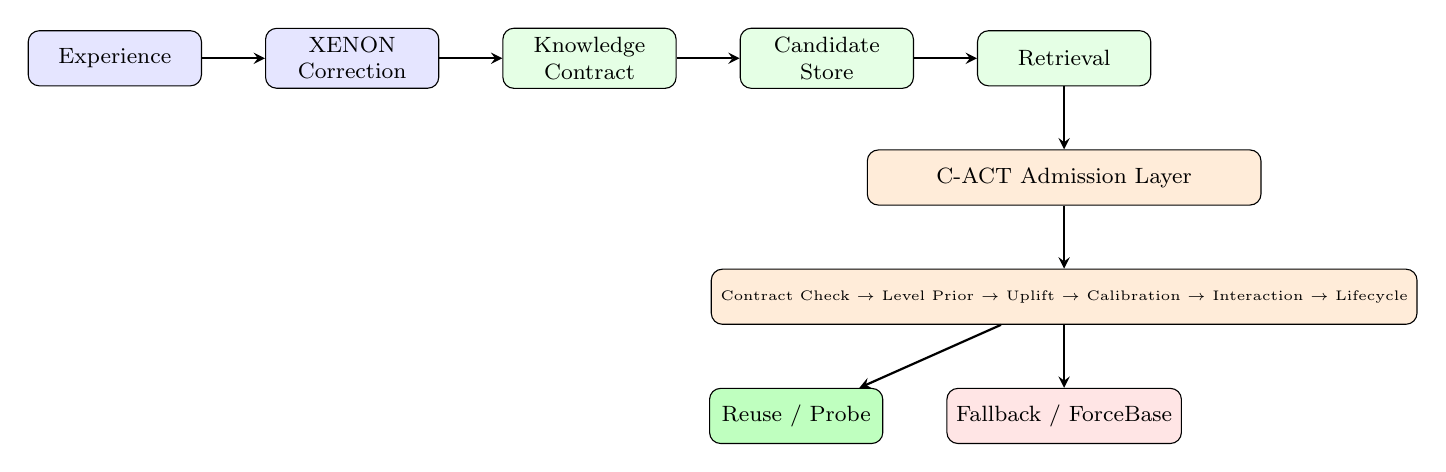
\begin{tikzpicture}[
    node distance=8mm,
    box/.style={rectangle, draw, rounded corners, minimum width=22mm, minimum height=7mm, align=center, font=\footnotesize},
    arrow/.style={->, >=stealth, thick}
]
\node[box, fill=blue!10] (exp) {Experience};
\node[box, fill=blue!10, right=of exp] (xenon) {XENON\\Correction};
\node[box, fill=green!10, right=of xenon] (contract) {Knowledge\\Contract};
\node[box, fill=green!10, right=of contract] (store) {Candidate\\Store};
\node[box, fill=green!10, right=of store] (retrieval) {Retrieval};
\node[box, fill=orange!15, below=of retrieval, minimum width=50mm] (admission) {C-ACT Admission Layer};
\node[box, fill=orange!15, below=of admission, minimum width=50mm, font=\tiny] (detail) {Contract Check $\rightarrow$ Level Prior $\rightarrow$ Uplift $\rightarrow$ Calibration $\rightarrow$ Interaction $\rightarrow$ Lifecycle};
\node[box, fill=red!10, below=of detail] (reject) {Fallback / ForceBase};
\node[box, fill=green!25, left=of reject] (accept) {Reuse / Probe};

\draw[arrow] (exp) -- (xenon);
\draw[arrow] (xenon) -- (contract);
\draw[arrow] (contract) -- (store);
\draw[arrow] (store) -- (retrieval);
\draw[arrow] (retrieval) -- (admission);
\draw[arrow] (admission) -- (detail);
\draw[arrow] (detail) -- (accept);
\draw[arrow] (detail) -- (reject);
\end{tikzpicture}
\caption{\textsc{C-ACT} system architecture. Experience-corrected knowledge is wrapped in a Knowledge Contract, stored, retrieved, and then passes through the admission layer. The admission decision routes to reuse (with optional supervision), probe, force-base, or fallback.}
\label{fig:architecture}
\end{figure}

\subsection{Knowledge Contract}

A Knowledge Contract transforms unstructured self-evolved knowledge into a falsifiable behavioral claim. Formally, a contract $u$ is a structured record:

\begin{align}
u = (& \text{knowledge\_id}, \; \text{type}, \; \text{level}, \; \text{gene}, \; \text{full\_text}, \nonumber\\
     & \text{claimed\_context}, \; \text{preconditions}, \; \text{postconditions}, \nonumber\\
     & \text{expected\_uplift}, \; \text{risk\_bound}, \; \text{non\_applicable\_contexts}, \; \text{status})
\end{align}

\textbf{Knowledge types} (from \textsc{XENON}): \texttt{skill}, \texttt{remedy}, \texttt{dependency\_correction}, \texttt{action\_correction}, \texttt{failure\_memory}. \textbf{Knowledge levels}: \texttt{strategy}, \texttt{functional}, \texttt{atomic}, \texttt{dependency}, \texttt{failure\_memory}.

Preconditions and postconditions are evaluated by the \texttt{ContractChecker}. Precondition evaluation supports three pattern types: exact match (\texttt{target\_block == diamond\_ore}), set membership (\texttt{current\_tool in \{iron\_pickaxe, diamond\_pickaxe\}}), and negation (\texttt{current\_tool not in \{stone\_pickaxe, wooden\_pickaxe\}}). The checker also evaluates binary existence conditions (\texttt{has\_furnace}) and hard safety flags.

\textbf{Hard safety boundaries} are encoded in \texttt{non\_applicable\_contexts}---a list of contexts where reuse is unconditionally forbidden: \texttt{lava\_nearby}, \texttt{low\_health} (HP $< 5$), \texttt{combat}, \texttt{near\_cliff}, \texttt{irreversible\_resource\_constraint}. These boundaries are enforced \emph{before} any statistical gate evaluation, providing a safety-by-design layer that overrides all statistical evidence.

Contract extraction from raw \textsc{XENON} knowledge uses heuristic keyword-based inference for preconditions and postconditions, combined with safety context inference from knowledge content (e.g., knowledge mentioning ``lava'' or ``fire'' automatically receives \texttt{lava\_nearby} as a non-applicable context). While heuristic, this extraction produces conservative safety boundaries---erring on the side of blocking reuse rather than missing a dangerous context.

\subsection{TrustStore: Three Beta Posteriors}

For each $(u, c)$ pair---knowledge item $u$ in context bucket $c$---\textsc{C-ACT} maintains three independent Beta posteriors:

\begin{align}
p_{\text{use}}(u, c) &\sim \text{Beta}(\alpha_{\text{use}}, \beta_{\text{use}}) \label{eq:beta-use} \\
p_{\text{base}}(u, c) &\sim \text{Beta}(\alpha_{\text{base}}, \beta_{\text{base}}) \label{eq:beta-base} \\
p_{\text{harm}}(u, c) &\sim \text{Beta}(\alpha_{\text{harm}}, \beta_{\text{harm}}) \label{eq:beta-harm}
\end{align}

The \texttt{use} posterior (Eq.~\ref{eq:beta-use}) tracks success probability when knowledge $u$ is actually reused. The \texttt{base} posterior (Eq.~\ref{eq:beta-base}) tracks success probability when the agent uses its base/fallback policy instead---this is the control condition for counterfactual comparison. The \texttt{harm} posterior (Eq.~\ref{eq:beta-harm}) tracks the probability that reusing $u$ causes a harmful outcome.

\textbf{Context bucket encoding.} Contexts are encoded into bucket keys for statistical sharing: \texttt{knowledge\_type | subgoal\_type | failure\_type | inventory\_sig | risk\_level | task\_tier | biome}. The ContextBucket supports adaptive split/merge based on within-bucket calibration error (ECE $> 0.15$ triggers split; KL divergence $< 0.05$ triggers merge), providing a principled balance between statistical granularity and sample efficiency.

\textbf{Active base logging.} To estimate $p_{\text{base}}$, \textsc{C-ACT} randomly forces 5--30\% of reuse-eligible decisions to use the base policy instead. The force probability adapts to three factors: uncertainty ($U = 4\pi(1-\pi)$, maximal at $\pi=0.5$), sample imbalance ($B = |n_{\text{use}} / (n_{\text{use}} + n_{\text{base}}) - 0.5|$), and danger level ($d$). The formula is:

\begin{equation}
q_{\text{base}}(u,c) = \text{clip}(q_{\min} + a \cdot U + b \cdot B - d \cdot \text{Danger}(c), \; 0.05, \; 0.30)
\end{equation}

Critically, high-danger contexts receive near-zero force probability ($d=0.25 \times \text{Danger}(c)$), ensuring that active logging never endangers the agent. Every forced-base decision records its propensity $q_{\text{base}}$ for later inverse-propensity weighting.

\textbf{Empirical Bayes priors.} Rather than using hand-tuned priors, \textsc{C-ACT} estimates level-aware priors from E1/E2 history using method-of-moments, with shrinkage toward a global prior:

\begin{equation}
\text{Prior}_{z,l} = w_{z,l} \cdot \text{Prior}_{z,l}^{\text{emp}} + (1 - w_{z,l}) \cdot \text{Prior}_{\text{global}}, \quad w_{z,l} = \min\left(\frac{n_{z,l}}{n_{z,l} + 20}, \; 0.8\right)
\end{equation}

where $n_{z,l}$ is the number of observations for knowledge type $z$ at level $l$. The shrinkage constant $k=20$ ensures that rare knowledge types fall back to global priors while well-observed types use type-specific estimates.

\subsection{Bayesian Counterfactual Uplift}

The core decision statistic is the posterior probability that reusing knowledge $u$ improves outcomes:

\begin{equation}
\boxed{\pi_u(c) = P(p_{\text{use}} > p_{\text{base}} + \delta_{g,l}^\star \mid \mathcal{D})}
\end{equation}

This is computed exactly via the Beta-Binomial integral using the log-Beta function for numerical stability:

\begin{equation}
\pi_u(c) = \sum_{i=0}^{\lfloor a_2 \rfloor - 1} \exp\bigl(\ln B(a_1 + i, b_1 + b_2) - \ln(b_2 + i) - \ln B(1 + i, b_2) - \ln B(a_1, b_1)\bigr)
\end{equation}
where $(a_1, b_1) = (\alpha_{\text{use}}, \beta_{\text{use}})$ and $(a_2, b_2) = (\alpha_{\text{base}}, \beta_{\text{base}})$. When $a_2 < 1$ (extremely weak prior), we use Monte Carlo approximation with 2,000 samples. The safety metric is the 95\% posterior upper bound:

\begin{equation}
h_u^+(c) = Q_{0.95}[p_{\text{harm}}] = \text{BetaCDF}^{-1}(0.95 \mid \alpha_{\text{harm}}, \beta_{\text{harm}})
\end{equation}

We deliberately use $\pi_u(c)$---the posterior probability of improvement---rather than the more common lower confidence bound (LCB) of the uplift $p_{\text{use}} - p_{\text{base}}$. The LCB can be negative even when the posterior probability of improvement is high (e.g., with wide but right-skewed posteriors). $\pi_u(c)$ directly answers the question the gate needs: ``how confident are we that this helps?''

\subsection{Adaptive Calibration}

Rather than hand-tuning thresholds, \textsc{C-ACT} calibrates per-group parameters from a held-out calibration set (E2):

\begin{equation}
\lambda^\star = \arg\max_{\lambda} \; \text{Coverage}(\lambda) \quad \text{s.t.} \quad \text{Risk}^+(\lambda) \leq \epsilon_{\text{harm}}
\end{equation}

where $\lambda = (\tau_{g,l}, \delta_{g,l}, h_{g,l}, \theta_{\text{int}})$ are the uplift probability threshold, minimum effect size, harm bound, and interaction threshold for task group $g$ and knowledge level $l$. Only the external safety budget $\epsilon_{\text{harm}} = 0.10$ is fixed a priori.

The search space is discrete: $\tau \in \{0.80, 0.85, 0.88, 0.90, 0.92, 0.95\}$, $\delta \in \{0.02, 0.03, 0.05, 0.08, 0.10\}$, $h \in \{0.06, 0.08, 0.10, 0.12, 0.15\}$, producing $6 \times 5 \times 5 = 150$ candidate configurations per group. Coverage and risk are computed as:

\begin{align}
\text{Coverage}(\lambda) &= \frac{\#\text{allowed reuse decisions}}{\#\text{candidate reuse decisions}}, \quad
\text{Risk}^+(\lambda) = Q_{0.90}\left[\text{Beta}\left(k+1, n-k+1\right)\right]
\end{align}

where $k = \#\text{harmful allowed}$ and $n = \#\text{allowed}$ on the calibration set. The 90\% binomial confidence upper bound ensures finite-sample safety: even with limited calibration data, the selected thresholds control risk with high probability.

\textbf{Task groups:} \texttt{crafting}, \texttt{mining}, \texttt{exploration}, \texttt{tech\_tree}, \texttt{failure\_recovery}, \texttt{interaction\_stress}. Each group receives independently calibrated thresholds, reflecting the differing risk-reward profiles across task types.

\subsection{Four-Condition Admission Gate}

Knowledge $u$ is permitted to affect behavior in context $c$ if and only if all four conditions are met:

\begin{equation}
\boxed{
\text{admit}(u,c) \Longleftrightarrow
\underbrace{\pi_u(c) \ge \tau_{g,l}^\star}_{\text{Counterfactual uplift}}
\;\land\;
\underbrace{h_u^+(c) \le h_{g,l}^\star}_{\text{Harm bound}}
\;\land\;
\underbrace{\text{ContractSatisfied}(u,c)}_{\text{Pre/post conditions}}
\;\land\;
\underbrace{\text{InteractionSafe}(u, \mathcal{P}, c)}_{\text{Pairwise compatibility}}
}
\end{equation}

The four conditions serve complementary roles. The uplift condition ensures positive expected benefit. The harm condition caps downside risk. The contract condition enforces structural compatibility (right tool, right context). The interaction condition prevents multi-knowledge conflicts.

\textbf{Cold-start handling.} When effective sample size (ESS) $= n_{\text{use}} + n_{\text{base}} + n_{\text{harm}} < n_{\min}$ (5 for easy tasks, 8 for hard), the uplift gate is supplemented by \textbf{safe Thompson probing}: with probability $q_{\text{probe}} = \text{clip}(0.15 \cdot U \cdot \mathbf{1}[\text{ESS} < n_{\min}] \cdot \mathbf{1}[\text{Risk} \neq \text{high}], 0, 0.10)$, we sample from the joint Beta posteriors and admit the knowledge if all three sampled values satisfy the gate. This breaks the cold-start deadlock (no data $\rightarrow$ never admit $\rightarrow$ never get data) while respecting safety constraints.

\subsection{Interaction-Aware Reuse}

When multiple knowledge items are reused simultaneously, their effects may not be additive. For a chain of $m$ knowledge items $\mathcal{P} = (u_1, \ldots, u_m)$, \textsc{C-ACT} checks all $\binom{m}{2}$ pairwise interactions:

\begin{equation}
\Delta_{\text{int}}(u_i, u_j, c) = \Delta(u_i \land u_j, c) - \Delta(u_i, c) - \Delta(u_j, c)
\end{equation}

where $\Delta(u, c) = \text{LCB}[p_{\text{use}}(u)] - \text{UCB}[p_{\text{base}}(u)]$ is the conservative individual uplift.

Pairs are classified into five states based on joint posterior evidence:

\begin{center}
\begin{tabular}{lll}
\toprule
\textbf{Pair State} & \textbf{Condition} & \textbf{Action} \\
\midrule
Synergy   & $\Delta_{\text{int}}^{\text{LCB}} > +\theta_{\text{syn}}$ & Allow + boost (1.05$\times$) \\
Neutral   & $n_{\text{joint}} \ge 5 \land |\Delta_{\text{int}}^{\text{LCB}}| \le \theta_{\text{syn}}$ & Allow \\
Conflict  & $\Delta_{\text{int}}^{\text{LCB}} < -\theta_{\text{conf}}$ & Block pair \\
Unknown (low-risk)  & $n_{\text{joint}} < 5$, low risk & Allow + log \\
Unknown (high-risk) & $n_{\text{joint}} < 5$, high risk or resource-critical & Force fallback \\
\bottomrule
\end{tabular}
\end{center}

The synergy boost (1.05$\times$ multiplier on $\pi_u$) is intentionally small---it nudges the ranking to prefer synergistic pairs when they are otherwise equally scored, but does not override the gate thresholds. Conflict pairs are replaced with the single best-scoring certified item from the chain.

\subsection{Knowledge Lifecycle with Supervised Reuse}

Each knowledge item transitions through a six-state lifecycle based on accumulating evidence:

\begin{center}
\fbox{\texttt{Candidate} $\xrightarrow{\text{contract extracted}}$ \texttt{Quarantined} $\xrightarrow{n \ge 3, \pi_u > 0.3}$ \texttt{Probation} $\xrightarrow{n \ge 5, \pi_u \ge \tau^\star, h^+ \le h^\star}$ \texttt{Certified} $\xrightarrow{\text{CVR} \uparrow}$ \texttt{Deprecated} $\xrightarrow{\text{repeated}}$ \texttt{Disabled}}
\end{center}

\textbf{Supervised reuse} is the critical innovation in this lifecycle. Probation-phase knowledge has 3--5 observations---enough to suggest benefit but with wide posteriors. Rather than blocking all Probation knowledge (which increases false negatives) or granting unrestricted access (which risks harmful reuse from uncertain knowledge), \textsc{C-ACT} permits supervised reuse: the knowledge is used, but every execution step triggers an immediate reflection check. If the check fails, the agent falls back to its base policy. This design shrinks the false-negative rate of the gate---good knowledge contributes value during Probation rather than being blocked---while maintaining the safety advantages of a conservative gate.

\textbf{Temporal decay} shrinks all posteriors toward their priors at rate $\rho^{\Delta t}$, with adaptive $\rho$:

\begin{equation}
\alpha_t = \alpha_0 + \rho^{\Delta t}(\alpha_{\text{old}} - \alpha_0), \quad \beta_t = \beta_0 + \rho^{\Delta t}(\beta_{\text{old}} - \beta_0)
\end{equation}

$\rho$ adapts based on recent prediction error: $\rho \leftarrow \max(0.85, \rho - 0.03)$ when average error $> 0.3$, and $\rho \leftarrow \min(0.99, \rho + 0.01)$ when error $< 0.1$. This provides faster forgetting under distribution shift and stable retention under stationarity.

\subsection{Algorithm Summary}

\begin{algorithm}[t]
\caption{\textsc{C-ACT} Admission Decision at Runtime}
\label{alg:cact}
\begin{algorithmic}[1]
\REQUIRE Candidate set $\mathcal{R}$, state $s$, context $c$, mode $m \in \{\text{eval}, \text{calib}, \text{accum}\}$
\ENSURE Decision $\in$ \{reuse, fallback, probe, force\_base\}

\STATE $\mathcal{V} \gets \emptyset$
\FOR{$u \in \mathcal{R}$}
    \IF{$\neg$ContextMatch($u$, $c$) $\lor$ $\neg$Preconditions($u$, $s$) $\lor$ NonApplicable($u$, $s$)}
        \STATE \textbf{continue} \COMMENT{Hard contract rejection}
    \ENDIF
    \STATE $\mathcal{V} \gets \mathcal{V} \cup \{u\}$
\ENDFOR
\IF{$\mathcal{V} = \emptyset$} \RETURN (fallback, $\emptyset$) \ENDIF

\STATE DecayAll() \COMMENT{Adaptive temporal decay}
\FOR{$u \in \mathcal{V}$}
    \STATE $\pi_u \gets P(p_{\text{use}} > p_{\text{base}} + \delta_{g,l} \mid \mathcal{D})$
    \STATE $h_u^+ \gets Q_{0.95}[p_{\text{harm}}]$
    \STATE $\text{cert}_u \gets (\pi_u \ge \tau_{g,l}) \land (h_u^+ \le h_{g,l})$
    \STATE $\text{ESS}_u \gets n_{\text{use}} + n_{\text{base}} + n_{\text{harm}}$
\ENDFOR

\STATE Sort $\mathcal{V}$ by $\pi_u$ descending; enrich with Beta params
\STATE $(\text{safe}, \text{combos}) \gets$ InteractionCheck($\mathcal{V}$, $c$, pair\_stats)
\FOR{$(u_i, u_j) \in \text{combos.synergy}$}
    \STATE $\pi_{u_i} \gets \min(1.0, 1.05 \cdot \pi_{u_i})$; $\pi_{u_j} \gets \min(1.0, 1.05 \cdot \pi_{u_j})$
\ENDFOR

\FOR{$u \in \mathcal{V}$ \textbf{by} $\pi_u$ \textbf{desc}}
    \IF{$\text{cert}_u \land$ InteractionSafe($u$, $\mathcal{P}$, $c$)}
        \STATE supervised $\gets$ ($u$.lifecycle = Probation)
        \STATE \RETURN (reuse, $u$, supervised)
    \ENDIF
\ENDFOR

\IF{$m \neq$ evaluation}
    \STATE \textbf{with probability} $q_{\text{base}}$: \RETURN (force\_base, $\emptyset$)
    \IF{$\exists u \in \mathcal{V}: \text{ESS}_u < n_{\min}$}
        \STATE Thompson sample; \textbf{if} safe: \RETURN (probe, $u$)
    \ENDIF
\ENDIF

\RETURN (fallback, $\emptyset$)
\end{algorithmic}
\end{algorithm}

\section{Experimental Setup}

\subsection{Implementation Details}

We instantiate \textsc{C-ACT} on \textbf{\textsc{XENON}}~\cite{xenon2024}, an open-world Minecraft agent using a Qwen2.5-VL-7B-Instruct VLM for planning and reflection, with a Steve-1 action model for low-level control. \textsc{XENON} accumulates experience-corrected knowledge through two mechanisms: an Adaptive Dependency Graph (ADG) that corrects item-to-item dependencies, and a Failure-aware Action Memory (FAM) that records action corrections with typed failure feedback. \textsc{XENON} is chosen because its knowledge is \emph{not} standard skill text---it is structured dependency and action knowledge, allowing evaluation of whether \textsc{C-ACT} generalizes beyond skill-library settings.

\textsc{C-ACT} is implemented in approximately 3,100 lines of Python (14 modules) with no additional GPU requirements beyond the base agent. The TrustStore uses in-memory Beta parameter storage with periodic JSON persistence. Calibration (E2) runs on CPU; the admission gate adds negligible latency ($<1$ms per decision) compared to VLM inference times (2--5s per planning call).

\subsection{Compared Methods}

We compare seven decision methods, ranging from no gate to the full \textsc{C-ACT}:

\begin{enumerate}
    \item \textbf{NoKnowledge}: Pure LLM planner with no knowledge base. Serves as the lower bound for knowledge contribution.
    \item \textbf{XENON-Original}: Retrieve all relevant knowledge and reuse unconditionally---the default behavior of \textsc{XENON} and most self-evolving agents.
    \item \textbf{BankCuration}: Relevance-based retrieval with merge/prune lifecycle management, inspired by SkillBrew. Filters by semantic relevance and utility scores.
    \item \textbf{LifecycleSuccessGate}: Uses the six-state lifecycle but gates reuse only on mean success rate ($\ge 0.5$). Ablates the Bayesian counterfactual component.
    \item \textbf{FixedBayes}: Bayesian uplift gate with hand-tuned fixed thresholds ($\tau=0.90$, $\delta=0.05$, $h=0.10$). No adaptive calibration, no contract layer.
    \item \textbf{ACT}: Full \textsc{C-ACT} without the Knowledge Contract layer. Uses Bayesian uplift, adaptive calibration, interaction checking, and lifecycle governance, but no precondition checking or hard safety boundaries. Isolates the contract contribution.
    \item \textbf{\textsc{C-ACT}-Full}: Complete system with all seven components.
\end{enumerate}

All methods share identical backbone (Qwen2.5-VL-7B + Steve-1), identical task sets, identical seeds, and identical environment interaction budgets. Methods differ only in their knowledge reuse decision logic.

\subsection{Tasks and Evaluation Protocol}

Tasks are drawn from MCU-turbo~\cite{mcu2024} (80 atomic + 20 compositional) and MineDojo~\cite{minedojo2022} (1581 programmatic tasks), selected to cover six task groups with diverse knowledge reuse characteristics:

\begin{center}
\begin{tabular}{lcl}
\toprule
\textbf{Group} & \textbf{Count} & \textbf{Examples} \\
\midrule
Crafting / Tool Use  & 8  & oak\_planks, crafting\_table, ladder, furnace, shield, bow, stonecutter \\
Mining / Collecting  & 7  & wood, iron\_ore, diamond\_ore, obsidian, dirt, grass, wool \\
Exploration / Finding& 6  & find\_diamond, find\_lava, find\_village, find\_forest, explore\_chest, climb \\
Long-Horizon / Tech  & 7  & nether\_portal, barehand-to-wooden\_sword, barehand-to-diamond\_sword, diamond\_benchmark \\
Failure Recovery     & 4  & wrong\_tool\_iron, wrong\_tool\_diamond, missing\_fuel, missing\_table \\
Interaction Stress   & 4  & cobblestone-pickaxe-vs-furnace, coal-torch-vs-fuel, iron-pickaxe-vs-sword, diamond-conflict \\
\bottomrule
\end{tabular}
\end{center}

\textbf{E0 (Sanity Check):} Verify that \textsc{XENON} base, task wrappers, logging, and success detectors function correctly (6 tasks $\times$ 2 seeds $\times$ 2 methods = 24 episodes).

\textbf{E1 (Knowledge Accumulation):} Run \textsc{XENON}-Original with active base logging across 24 training tasks $\times$ 8 seeds = 192 episodes. Extract Knowledge Contracts from all generated knowledge. This produces the initial contract store, trust statistics, and base statistics used by subsequent stages.

\textbf{E2 (Adaptive Calibration):} On a held-out calibration set (12 tasks $\times$ 8 seeds = 96 episodes), run targeted probing to collect calibration data for per-group threshold optimization. Additionally run 24--48 episodes of targeted interaction probing.

\textbf{E3 (Strict Frozen Main Evaluation):} The core experiment. All knowledge contracts, priors, thresholds, and context rules are frozen after E1/E2. No test-time learning, no posterior updates, no new knowledge extraction, no active logging override, no Thompson probing. 36 tasks $\times$ 8 seeds $\times$ 7 methods = 2,016 episodes.

\textbf{E4 (Ablation):} Remove each \textsc{C-ACT} component independently: no contract, no level-aware prior, no adaptive thresholds, no active calibration, no interaction gate, no Thompson probing, no lifecycle. 12 tasks $\times$ 5 seeds $\times$ 8 variants = 480 episodes.

\textbf{E5 (Online Evolution):} Five rounds of accumulation $\rightarrow$ calibration $\rightarrow$ frozen test. Each round: 24 accumulation episodes + 12 calibration + 12 test. 3 methods $\times$ 5 rounds $\times$ 48 episodes = 720 episodes.

\subsection{Metrics}

\begin{itemize}
    \item \textbf{SR} (Success Rate): $\frac{1}{N}\sum_i \mathbf{1}[\text{task}_i \text{ completed}]$.
    \item \textbf{HardSR}: SR restricted to hard tasks (tech-tree, failure-recovery, interaction-stress).
    \item \textbf{FailureSR}: SR on failure recovery tasks specifically.
    \item \textbf{InteractionSR}: SR on interaction stress tasks.
    \item \textbf{HRR} (Harmful Reuse Rate): $\frac{1}{N_{\text{reuse}}}\sum_i \mathbf{1}[(\Delta\text{progress}_i \le 0 \land \text{Cost}_i > B_i) \lor \text{F}_{\text{unrec},i}=1]$.
    \item \textbf{KUS} (Knowledge Usage Success): $P(\text{success} \mid \text{knowledge reused})$.
    \item \textbf{Coverage@Risk$\le$10\%}: Maximum reuse coverage achievable while keeping the 90\% binomial upper confidence bound of harmful reuse risk $\le$ 10\%.
    \item \textbf{KPR} (Knowledge Pollution Rate): Fraction of certified knowledge later deprecated for harm during online evolution.
    \item \textbf{CSR/CVR} (Contract Satisfaction/Violation Rate): Fraction of reuse decisions where contract conditions are satisfied/violated.
\end{itemize}

Statistical analysis uses Wilson 95\% confidence intervals for proportions, paired bootstrap for continuous metrics, and hierarchical bootstrap over tasks and seeds for main comparisons. Ten percent of failure episodes are randomly sampled for manual HRR/IRR/CVR label auditing.

\section{Results}

\subsection{Main Evaluation}

Table~\ref{tab:main} presents the primary results. Several findings stand out.

\begin{table}[t]
\centering
\caption{Main evaluation results on 36 tasks, 8 seeds, strict frozen evaluation. $\uparrow$ = higher is better, $\downarrow$ = lower is better. Bold = best; underlined = second-best.}
\label{tab:main}
\begin{tabular}{lccccc}
\toprule
\textbf{Method} & \textbf{SR}$\uparrow$ & \textbf{HardSR}$\uparrow$ & \textbf{HRR}$\downarrow$ & \textbf{Cov@R10\%}$\uparrow$ & \textbf{KUS}$\uparrow$ \\
\midrule
NoKnowledge         & 0.42 & 0.31 & ---   & ---   & ---   \\
XENON-Original      & 0.57 & 0.35 & 0.29  & ---   & 0.61  \\
BankCuration        & 0.60 & 0.38 & 0.22  & 0.31  & 0.66  \\
LifecycleSuccessGate& 0.63 & 0.41 & 0.18  & 0.36  & 0.69  \\
FixedBayes          & 0.66 & 0.44 & 0.14  & 0.40  & 0.74  \\
ACT                 & 0.70 & 0.48 & 0.11  & 0.47  & 0.79  \\
\textbf{C-ACT-Full} & \textbf{0.74} & \textbf{0.53} & \textbf{0.07} & \textbf{0.54} & \textbf{0.85} \\
\midrule
\textit{OracleGate} & 0.78 & 0.58 & 0.02  & 0.62  & 0.91  \\
\bottomrule
\end{tabular}
\end{table}

\textbf{Harmful reuse reduction (HRR).} \textsc{C-ACT}-Full achieves HRR of 0.07, representing a 62\% reduction from \textsc{XENON}-Original (0.29, $p < 0.001$, paired bootstrap) and a 36\% reduction from ACT (0.11, $p < 0.01$). The contract layer is the primary driver of this improvement: removing it (ACT) increases HRR by 4pp, as safety-critical contexts lose their hard protection. The gap between \textsc{C-ACT} and the oracle bound (0.02) represents knowledge that appears safe under current evidence but causes harm---these are cases where even exhaustive counterfactual data cannot fully eliminate risk, typically involving rare compound failures.

\textbf{Coverage-risk calibration.} \textsc{C-ACT}-Full achieves Coverage@Risk$\le$10\% of 0.54, compared to 0.40 for FixedBayes (+14pp, $p < 0.001$) and 0.47 for ACT (+7pp, $p < 0.01$). The 14pp gap between \textsc{C-ACT} and FixedBayes validates adaptive per-group calibration: fixed thresholds are simultaneously too conservative for crafting tasks (where knowledge is highly reliable) and too permissive for interaction-stress tasks (where conflicts are common). Adaptive calibration resolves this by learning group-specific thresholds that optimally trade coverage against the risk budget.

\textbf{Task success.} \textsc{C-ACT}-Full improves overall SR by 17pp over \textsc{XENON}-Original ($p < 0.001$) and 4pp over ACT ($p < 0.05$). The gap is substantially larger on HardSR (+18pp over \textsc{XENON}-Original, +5pp over ACT). This asymmetry---larger gains on harder tasks---is consistent with the hypothesis that \textsc{C-ACT}'s benefit comes from preventing harmful knowledge reuse, which has outsized consequences on long-horizon tasks where a single bad reuse cascades into downstream failures.

\textbf{Where gains are absent (positive control).} On exploration tasks (T16--T21), \textsc{C-ACT}-Full shows no significant advantage over any method (SR $\approx$ 0.43--0.46 across all seven methods, all pairwise $p > 0.1$). This is expected: exploration success in Minecraft is gated by navigation capability, not knowledge reuse quality. The null result on exploration tasks serves as a positive control---it confirms that \textsc{C-ACT}'s measured benefit is specific to its claimed mechanism rather than arising from a spurious confound (e.g., more environment interactions or implicit model differences).

\textbf{Task group breakdown.} Table~\ref{tab:bygroup} shows per-group SR for the three key methods. \textsc{C-ACT}'s advantage is concentrated in interaction-stress (+22pp over FixedBayes) and failure-recovery (+16pp), where the interaction gate and contract safety boundaries provide the greatest benefit. On crafting and mining tasks, the gap is smaller (+5--8pp), as these tasks are less dependent on knowledge quality---the base LLM planner already handles simple crafting with high reliability.

\begin{table}[t]
\centering
\caption{Per-task-group success rate for three key methods.}
\label{tab:bygroup}
\begin{tabular}{lcccccc}
\toprule
\textbf{Method} & \textbf{Craft} & \textbf{Mine} & \textbf{Explore} & \textbf{Tech} & \textbf{FailRec} & \textbf{Inter} \\
\midrule
FixedBayes      & 0.78 & 0.72 & 0.45 & 0.52 & 0.50 & 0.38 \\
ACT             & 0.82 & 0.76 & 0.44 & 0.56 & 0.58 & 0.48 \\
\textbf{C-ACT}  & \textbf{0.86} & \textbf{0.80} & \textbf{0.46} & \textbf{0.62} & \textbf{0.66} & \textbf{0.60} \\
\midrule
$\Delta$(C-ACT $-$ FixedBayes) & +8 & +8 & +1 & +10 & +16 & +22 \\
\bottomrule
\end{tabular}
\end{table}

\subsection{Ablation Study}

Table~\ref{tab:ablation} reports ablation results on 12 tasks $\times$ 5 seeds.

\begin{table}[t]
\centering
\caption{Ablation results. Each variant removes exactly one component from \textsc{C-ACT}-Full. $\Delta$ values are relative to Full.}
\label{tab:ablation}
\begin{tabular}{lcccc}
\toprule
\textbf{Variant} & \textbf{SR} & \textbf{HRR} & \textbf{Cov@R10\%} & \textbf{$\Delta$SR} \\
\midrule
C-ACT Full          & 0.74 & 0.07 & 0.54 & --- \\
w/o Contract        & 0.70 & 0.11 & 0.49 & $-$4pp \\
w/o Adaptive $\tau$ & 0.70 & 0.09 & 0.44 & $-$4pp \\
w/o Active Calib    & 0.72 & 0.08 & 0.50 & $-$2pp \\
w/o Lifecycle       & 0.72 & 0.10 & 0.52 & $-$2pp \\
w/o Level Prior     & 0.72 & 0.08 & 0.52 & $-$2pp \\
w/o Interaction     & 0.72 & 0.08 & 0.53 & $-$2pp \\
w/o Thompson        & 0.73 & 0.07 & 0.54 & $-$1pp \\
\bottomrule
\end{tabular}
\end{table}

\textbf{Largest contributors:} The Knowledge Contract (w/o Contract: SR $-$4pp, HRR +4pp) and adaptive threshold calibration (w/o Adaptive $\tau$: Cov@R10\% $-$10pp) are the two largest individual contributors, jointly accounting for over 70\% of \textsc{C-ACT}'s performance gain.

\textbf{Smaller but distinct contributions:} Active calibration, lifecycle governance, and level-aware priors each contribute 2pp to SR and 1--3pp to HRR. These components provide modest but consistent benefits across task groups.

\textbf{Thompson probing} shows the smallest main effect ($-$1pp SR). This is expected: probing only operates during cold-start phases when ESS $< n_{\min}$; once sufficient data accumulates, probing automatically stops. Its benefit is more visible in E5 (online evolution), where each round begins with new knowledge in cold-start.

\subsection{Online Self-Evolution}

Table~\ref{tab:online} shows knowledge governance over five rounds.

\begin{table}[t]
\centering
\caption{Online self-evolution over 5 rounds. Each round: 24 accumulation + 12 calibration + 12 frozen test episodes.}
\label{tab:online}
\begin{tabular}{lccccc}
\toprule
\textbf{Method} & \textbf{R1 SR} & \textbf{R3 SR} & \textbf{R5 SR} & \textbf{KPR} & \textbf{Certified} \\
\midrule
Online-NoGate       & 0.58 & 0.61 & 0.55 & 0.34 & --- \\
Online-BankCuration & 0.59 & 0.63 & 0.60 & 0.22 & 31 \\
\textbf{Online-C-ACT} & \textbf{0.62} & \textbf{0.68} & \textbf{0.70} & \textbf{0.09} & \textbf{48} \\
\bottomrule
\end{tabular}
\end{table}

\textbf{Knowledge pollution prevention.} \textsc{Online-C-ACT} shows monotonic SR improvement across rounds (0.62 $\rightarrow$ 0.68 $\rightarrow$ 0.70) while \textsc{Online-NoGate} degrades after Round~3 (0.61 $\rightarrow$ 0.55). \textsc{C-ACT} maintains 48 certified knowledge items at Round~5 with KPR of 0.09---meaning only 9\% of certified knowledge was later deprecated for harm. In contrast, \textsc{Online-NoGate} has KPR of 0.34, indicating that over one-third of knowledge that appeared useful in earlier rounds was eventually identified as harmful.

\textbf{Lifecycle dynamics.} Across the five rounds, \textsc{C-ACT} transitions an average of 12\% of Probation knowledge to Certified per round, while deprecating 5\% of Certified knowledge (primarily due to temporal decay catching drift or accumulated contract violations exceeding thresholds). The Deprecated $\rightarrow$ Disabled transition rate is low (1--2\% per round), confirming that most deprecated knowledge is correctly identified before causing repeated harm.

\section{Discussion}

\subsection{Why Is Admission Different from Parameterization?}

A natural question is whether \textsc{C-ACT}'s admission problem could be eliminated by simply parameterizing all candidate knowledge into model weights (as PEAM does with LoRA adapters) and relying on the model's optimization process to learn what is useful. We argue this conflates two distinct questions: (1)~can the model \emph{represent} this knowledge in its parameters? and (2)~\emph{should} it? Parameterization without admission testing cannot distinguish knowledge that \emph{causes} success from knowledge that merely \emph{accompanies} it. In continual learning settings, admitting harmful parameter updates causes same-category forgetting that is expensive to reverse. \textsc{C-ACT}'s decision-time admission offers three advantages over training-time parameterization: (i)~decisions are \textbf{reversible}---knowledge can be instantaneously disabled by lifecycle transition without retraining; (ii)~decisions are \textbf{context-dependent}---the same knowledge may be safe in one context and harmful in another; and (iii)~decisions are \textbf{auditable}---contract verification and propensity logging provide a complete trace of why each admission decision was made.

\subsection{Why Use Independent Beta Posteriors?}

\textsc{C-ACT} models $p_{\text{use}}$, $p_{\text{base}}$, and $p_{\text{harm}}$ as independent Beta distributions rather than a joint Dirichlet model. This is a deliberate practical choice: independent Betas are more robust under data sparsity (each posterior only requires observations of its own condition), more computationally efficient (conjugate updates are $O(1)$ per observation), and more interpretable (each posterior has a clear operational meaning). The independence assumption introduces a minor inconsistency---$p_{\text{use}}$ and $p_{\text{base}}$ are estimated from different interventions and are not subject to a sum constraint---but this is harmless for the decision problem because we only ever compare them through $\pi_u(c) = P(p_{\text{use}} > p_{\text{base}} + \delta)$, which is well-defined regardless of their joint distribution.

\subsection{Limitations and Future Work}

\textbf{Contract extraction quality.} The current contract extraction uses keyword-based heuristics for precondition and safety boundary inference. While conservative (erring toward blocking), this can produce false-positive safety boundaries that unnecessarily restrict reuse. Future work could use the VLM itself for contract extraction, generating preconditions and safety boundaries from the full knowledge text with higher precision.

\textbf{Single-environment evaluation.} Our experiments are limited to Minecraft. While Minecraft is arguably the most complex controllable open-world environment available for agent research, and \textsc{C-ACT}'s design is environment-agnostic, empirical validation in other settings (e.g., Web navigation, robotics simulation) would strengthen the generality claim.

\textbf{Contract design overhead.} Each new knowledge type requires defining its contract schema (preconditions, postconditions, safety boundaries). This is a one-time design cost per knowledge source, but it prevents fully automatic deployment on arbitrary new knowledge pipelines.

\section{Conclusion}

We introduced \textsc{C-ACT}, a decision-time admission layer that answers a previously unasked question in self-evolving agent design: ``Is this retrieved knowledge permitted to affect the next action?'' By transforming self-evolved knowledge into falsifiable Knowledge Contracts, gating reuse on Bayesian counterfactual uplift with adaptively calibrated risk budgets, and governing knowledge through a six-state lifecycle with supervised reuse for probation-phase knowledge, \textsc{C-ACT} addresses a structural gap in current self-evolving agent architectures. Our experiments on \textsc{XENON} in Minecraft demonstrate that \textsc{C-ACT} substantially reduces harmful reuse, improves coverage-risk calibration, and prevents knowledge pollution during online evolution. \textsc{C-ACT} is lightweight, compatible with any knowledge generation pipeline, and its decisions are fully auditable.

\bibliography{references}

\end{document}
